\documentclass[12pt,a4paper]{article}
\usepackage{ucebnice}


\usepackage{scalerel}
\newlength\curht
\def\defaultdimfrac{.98}
\def\defaultstartht{\baselineskip}
\newcommand\diminish[2][\defaultdimfrac]{%
  \curht=\defaultstartht\relax
  \def\dimfrac{#1}%
  \diminishhelpA{#2}%
}
\newcommand\diminishhelpA[1]{%
  \expandafter\diminishhelpB#1\relax%
}
\def\diminishhelpB#1#2\relax{%
  \scaleto{\strut#1}{\curht}%
  \curht=\dimfrac\curht\relax%
  \ifx\relax#2\relax\else\diminishhelpA{#2}\fi%
}
\def\pinum{3,14159265358979323846264338327950288419716939937510}
\def\eunum{2,71828182845904523536028747135266249775724709369995}

\title{Základní matematické poznatky}
\author{Ondřej Škubala}
\date{\today}

\begin{document}

\maketitle
\newpage


\section{Číselné obory}

\begin{quotebox}
{„Bůh stvořil přirozená čísla; všechno ostatní je dílo člověka.“}
{Leopold Kronecker}
\end{quotebox}

Čísla provázejí lidstvo od nejstarších dob. Nejprve sloužila k jednoduchému
počítání předmětů a vyjádření množství. Postupem času lidé zjistili, že
k řešení složitějších problémů – například při dělení, měření nebo obchodování – 
je třeba čísla nově definovat a rozšířit jejich původní množinu. 

K tomu abychom si mohli říct, co je číslo musíme napřed ujastnit rozdíl mezi číslem a číslicí:

\begin{definitionbox}
\textbf{Číslo} je abstraktní matematický pojem, který vyjadřuje velikost, množství
nebo pořadí.\\
\textbf{Cifra} je znak, kterým číslo zapisujeme. V desítkové soustavě máme deset
cifer: 0–9.
\end{definitionbox}

\begin{examplebox}
Číslo deset zapisujeme dvěma ciframi: „1“ a „0“. Číslo dvacet pět zapisujeme dvěmi ciframi: „2“ a „5“.
\end{examplebox}


K vyjádření čísel používáme různé způsoby zápisu – tzv. \textbf{číselné soustavy}.  
Rozlišujeme:

\begin{itemize}
    \item \important{nepoziční soustavy} – hodnota symbolu (znaku) závisí pouze na samotném symbolu, nikoli na jeho místě v čísle.
    \item \important{poziční soustavy} – hodnota čísla závisí na pozici číslice i na základu (bázi) soustavy.
\end{itemize}

\begin{definitionbox}
\textbf{Nepoziční soustava} je taková soustava, kde každý znak má pevnou hodnotu, nezávislou na své pozici.  
Příklad: římské číslice, nebo jedničková soustava – např. zápisem třech značek „ | | | “ (nebo tří čárek) vyjádříme číslo tři.  
\end{definitionbox}
\newpage
\begin{definitionbox}
\textbf{Poziční soustava} je charakterizována \important{základem} (radix), což je kladné celé číslo definující, kolik různých číslic (včetně nuly) může být v soustavě použito.  
Číslo v poziční soustavě s základem \(b\) a ciframi \(a_k a_{k-1} \dots a_1 a_0\) odpovídá hodnotě:
\[
a_k b^k + a_{k-1} b^{k-1} + \dots + a_1 b^1 + a_0 b^0,
\]
kde každá cifra \(a_i\) splňuje \(0 \le a_i < b\).  
\end{definitionbox}


Mezi běžné poziční soustavy patří: 
      \begin{itemize}
         \item dvojková (\(b=2\)), 
         \item trojková (\(b=3\)),
         \item osmičková (\(b=8\)), 
         \item desítková (\(b=10\)), 
         \item dvanáctková (\(b=12\)), 
         \item šestnáctková (\(b=16\)), 
         \item šedesátková (\(b=60\)),  
      \end{itemize}
V takových soustavách může být číslo zapsáno se zlomkovou částí – části se oddělují desetinnou čárkou či tečkou.  


\begin{examplebox}
Příklad převodu a zápisu:
\begin{align*}
25_{10} &= 11001_2 = 31_8 = 19_{16} \\
3B0F_{16} &= 3 \cdot 16^3 + 11 \cdot 16^2 + 0 \cdot 16^1 + 15 \cdot 16^0 = 15119_{10}
\end{align*}
\end{examplebox}

Tento úvod do čísel a jejich zápisů nás přirozeně vede k další kapitole –
\textbf{číselným oborům}, které budeme postupně poznávat.

\newpage
\subsection{Druhy číselných oborů}

Číselné obory vznikaly postupně jako rozšíření množiny přirozených čísel $\mathbb{N}$.
Každý nový obor umožňuje řešit úlohy, které v předchozím oboru řešit nelze.
Než se pustíme do jednotlivých číselných oborů podrobněji, shrňme si nejprve jejich základní vlastnosti:

\begin{center}
\arrayrulecolor{tableborder}
\newcolumntype{M}[1]{>{\centering\arraybackslash}m{#1}}
\begin{tabular}{|M{5cm}|M{9,5cm}|}
\hline
\rowcolor{pastelblue!80} \textbf{Obor čísel} & \textbf{Co vyjadřují} \\
\hline
\makecell{\textbf{Přirozená čísla} \\ $1,2,3,4,\dots$} & Slouží k vyjádření počtu osob, zvířat, předmětů apod. \\
\hline
\makecell{\textbf{Celá čísla} \\ $\dots,-2,-1,0,1,2,\dots$} & Vyjadřují počty, dluhy a záporné změny \\
\hline
\makecell{\textbf{Racionální čísla} \\ $\tfrac{1}{2}, -\tfrac{3}{5}, 7$} & Umožňují vyjadřovat části celku, poměry, zlomky \\
\hline
\makecell{\textbf{Iracionální čísla} \\ $\sqrt{2}, \pi, e$} & Čísla, která nelze vyjádřit jako zlomek; nekonečný neperiodický desetinný rozvoj \\
\hline
\makecell{\textbf{Reálná čísla} \\ $-3, 0, \tfrac{1}{2}, \pi$} & Spojitá měření na číselné ose, vzdálenosti \\
\hline
\makecell{\textbf{Imaginární čísla} \\ $i, -2i, \tfrac{1}{3}i$} & Odmocniny ze záporných čísel \\
\hline
\makecell{\textbf{Komplexní čísla} \\ $2+3i, -i$} & Řešení rovnic, použití ve fyzice a elektrotechnice \\
\hline
\end{tabular}
\arrayrulecolor{black}
\end{center}

Pro číselné množiny se používá následující označení:
\begin{definitionbox}
\begin{itemize}
    \item $\mathbb{N}$ – množina všech \important{přirozených čísel},
    \item $\mathbb{Z}$ – množina všech \important{celých čísel},
    \item $\mathbb{Q}$ – množina všech \important{racionálních čísel},
    \item $\mathbb{R}$ – množina všech \important{reálných čísel},
    \item $\mathbb{C}$ – množina všech \important{komplexních čísel}.
\end{itemize}
\end{definitionbox}

Toto ovšem nejsou veškeré číselné obory. Existují například i \important{hyperkomplexní čísla}, 
která mají velice úzké využití (např. v počítačové grafice a fyzice).  
V běžné matematice se však vystačíme s obory uvedenými výše.

Zároveň se v praxi a v průběhu studia matematiky určitě ještě setákem s \important{odvozenými množinami číselných oborů}, 
tzv. „deriváty oborů“. Ty se zapisují pomocí horních nebo dolních indexů:
\begin{itemize}
    \item $\mathbb{N}_0$ – množina přirozených čísel rozšířená o nulu,
    \item $\mathbb{Z}^-$ – množina všech záporných celých čísel,
    \item $\mathbb{R}^+$ – množina všech kladných reálných čísel,
    \item $\mathbb{R}_0^+$ – množina všech nezáporných reálných čísel (kladná čísla a nula).
\end{itemize}

\begin{notebox}
Přirozená čísla lze formálně definovat pomocí tzv. 
\important{Peanových axiomů}. Ty zavádějí nulu, pojem „následníka“ čísla
a určují základní vlastnosti přirozených čísel, například že každé číslo má
jednoznačného následníka a že nula není následníkem žádného čísla.
\end{notebox}

\begin{definitionbox}
Jsou-li v množině čísel určitého druhu definovány operace \important{sčítání} a 
\important{násobení}, pak mluvíme o \important{číselném oboru}.
\end{definitionbox}

\section{Přirozená čísla}
\begin{historicalbox}
\textbf{Krátký exkurz do historie čísel:}  

První důkazy o používání čísel nacházíme už v pravěku – lidé si pomáhali jednoduchými značkami, například 
zářezem na kosti nebo dřevěné holi, aby vyjádřili počet ulovených zvířat. Jedním z nejznámějších důkazů 
je tzv. \textit{Išango kost} z Afriky (cca 20 000 př. n. l.), na které jsou patrné soustavy zářezů připomínající 
prvotní aritmetiku.  

Staří Sumerové a Babyloňané vyvinuli poziční \textbf{šedesátkovou soustavu}, jejíž stopy přežívají dodnes 
– například v rozdělení hodiny na 60 minut a kruhu na 360°.  
Řekové a Římané naopak používali \textbf{nepoziční soustavy}: řecká čísla byla odvozena z písmen abecedy, 
Římané nám zanechali dodnes známé symboly I, V, X, L, C, D, M.  

Současné „arabské“ číslice (0–9), které denně používáme, mají původ v \textbf{indické matematice}. 
Do Evropy se dostaly prostřednictvím arabských učenců ve středověku a postupně nahradily římský systém, 
který byl pro větší počty velmi nepraktický.  

Vývoj čísel tedy nebyl přímočarý – vznikaly různé systémy podle potřeb dané kultury. 
Teprve sjednocení a převzetí arabských číslic umožnilo rozvoj moderní matematiky, jak ji známe dnes.
\end{historicalbox}


Množina přirozených čísel $\mathbb{N}$ tvoří základ celého číselného systému. 
Je možné ji formálně definovat například pomocí \important{Peanových axiomů}, 
které zavádějí číslo nula, pojem „následníka“ čísla a určují základní vlastnosti 
přirozených čísel. V běžné matematice si však přirozená čísla můžeme 
představit jednoduše jako čísla $1, 2, 3, \dots$, která používáme k počítání.

\begin{notebox}
Přirozená čísla tvoří základ každodenního počítání – označují počet předmětů nebo osob, 
například „ve třídě je 28 žáků“ či „na polici stojí 12 knih“. Avšak již už zde nepatří „rozdíl 3 a 7“.
\end{notebox}

\newpage

Na množině přirozených čísel jsou definovány dvě základní operace – 
\important{sčítání} a \important{násobení}. 
Tyto operace splňují několik důležitých vlastností, které lze shrnout následovně:

\begin{definitionbox}
Pro každá tři přirozená čísla $a, b, c \in \mathbb{N}$ platí následující vlastnosti:

\begin{tabular}{p{5cm} p{4cm} p{2cm}}

$a+b \in \mathbb{N}$ & $a \cdot b \in \mathbb{N}$ & \hfill(U) \\
$a+(b+c) = (a+b)+c$ & $a \cdot (b \cdot c) = (a \cdot b)\cdot c$ & \hfill(A) \\
$a+b = b+a$ & $a \cdot b = b \cdot a$ & \hfill(K) \\
 & $a \cdot 1 = a$ & \hfill(N)\\
\multicolumn{2}{c}{ $a \cdot (b+c) = a\cdot b + a\cdot c$ } & \hfill(D) \\
\end{tabular}
\end{definitionbox}

Všimněte si nápadné obdoby sčítání a násobení zapsaných v prních třech operacích. Označení v posledním sloupci znamená:

\noindent
\begin{itemize}
    \item (U) \textbf{Uzavřenost} – součtem dvou přirozených čísel je opět číslo přirozené.
    \item (A) \textbf{Asociativita} – nezáleží na na pořadí, výsledek je vždy stejný.
    \item (K) \textbf{Komutativita} – pořadí sčítanců nebo činitelů nemá vliv na výsledek.
    \item (N) \textbf{Neutrální prvek} – číslo 1 je neutrální prvek vzhledem k násobení.
    \item (D) \textbf{Distributivita} – násobení se „roznásobí“ přes součet: $a\cdot(b+c)=a\cdot b+a\cdot c$.
\end{itemize}

\begin{examplebox}
\textbf{Příklady z oboru přirozených čísel:}

\begin{itemize}
    \item Rozdíl čísel $7$ a $2$ (v tomto pořadí) je číslo $5$, protože platí $2+5=7$. Výsledek tedy náleží do $\mathbb{N}$.
    \item Podíl čísel $15$ a $5$ je $3$, protože $5 \cdot 3 = 15$. Také tento výsledek patří do $\mathbb{N}$.
    \item Mocnina $3^5$ znamená $3 \cdot 3 \cdot 3 \cdot 3 \cdot 3$, což je $243$. Výsledek zůstává v $\mathbb{N}$.
    \item Rozdíl čísel $3$ a $7$ (v tomto pořadí) je $-4$, protože $7 + (-4) = 3$. Takový výsledek však \textbf{nepatří} do $\mathbb{N}$.
    \item Podíl čísel $5$ a $15$ je $\tfrac{1}{3}$, neboť $15 \cdot \tfrac{1}{3} = 5$. Ani tento výsledek \textbf{nepatří} do $\mathbb{N}$.
\end{itemize}
\end{examplebox}

\newpage

\section{Celá čísla}

\begin{historicalbox}
\textbf{Jak vznikla záporná čísla?}  

Myšlenka záporných čísel se objevuje až dlouho po přirozených číslech.  
Ve starověkém Řecku byla záporná čísla odmítána – řečtí matematici považovali čísla výhradně za „počty“ věcí, 
a tak se jim zdála záporná čísla nesmyslná. Proto ve většině jejich spisů najdeme jen kladná čísla a nulu.  

Naopak v Indii a Číně byla záporná čísla už ve starověku využívána. Indičtí matematici je chápali jako „dluhy“, 
zatímco kladná čísla označovala „majetek“. Čínské texty obsahují návody na počítání se zápornými čísly pomocí 
červených (kladných) a černých (záporných) kamínků.

\smallskip
Do Evropy pronikla záporná čísla přes arabskou matematiku, avšak ještě v renesanci byla přijímána s nedůvěrou.  
Například francouzský matematik René Descartes v 17. století nazýval záporné výsledky „falešnými kořeny“ rovnic.  

Teprve s rozvojem algebry a analytické geometrie se ukázalo, že bez záporných čísel nelze popsat řadu problémů – 
například pohyb v protisměru, teploty pod nulou nebo řešení lineárních rovnic.  
Od té doby se stala záporná čísla (a tedy i množina celých čísel) plnohodnotnou součástí matematiky.  

\end{historicalbox}


Množina celých čísel se označuje symbolem $\mathbb{Z}$ (z německého \textit{Zahlen} = čísla).  
Zahrnuje všechna přirozená čísla, jejich záporné protějšky a navíc také nulu:
\[
\mathbb{Z} = \{ \dots, -3, -2, -1, 0, 1, 2, 3, \dots \}
\]

Zavedení záporných čísel nám umožnilo řešit úlohy, které v oboru přirozených čísel řešit nešlo – 
například rozdíl $3-7$ či rovnice typu $x+5=2$.

\begin{notebox}
Celá čísla používáme běžně v životě, když popisujeme změny stavu – například teplotu ($-5^\circ$\,C), 
výškovou polohu (300 m n. m. vs. 50 m pod hladinou moře) nebo finanční situaci (zisk +200 Kč, dluh –150 Kč).
\end{notebox}

Na množině celých čísel jsou definovány čtyři základní operace – sčítání, odčítání, násobení a dělení.  
První tři splňují stejné vlastnosti jako v $\mathbb{N}$, ovšem s tím rozdílem, že nyní existuje i 
\important{neutrální prvek pro sčítání} a \important{opačné číslo}. 

\begin{definitionbox}
Pro každá tři celá čísla $a, b, c \in \mathbb{Z}$ platí následující vlastnosti:

\begin{tabular}{p{5cm} p{4cm} p{2cm}}
$a+b \in \mathbb{Z}$ & $a \cdot b \in \mathbb{Z}$ & \hfill(U) \\
$a+(b+c) = (a+b)+c$ & $a \cdot (b \cdot c) = (a \cdot b)\cdot c$ & \hfill(A) \\
$a+b = b+a$ & $a \cdot b = b \cdot a$ & \hfill(K) \\
$a+0 = a$ & $a \cdot 1 = a$ & \hfill(N) \\
$a + (-a) = 0$ & – & \hfill(O) \\
\multicolumn{2}{c}{ $a \cdot (b+c) = a\cdot b + a\cdot c$ } & \hfill(D) \\
\end{tabular}
\end{definitionbox}

\noindent
\begin{itemize}
    \item (U) \textbf{Uzavřenost} – výsledek je vždy celé číslo.  
    \item (A) \textbf{Asociativita} – nezáleží na seskupení členů.  
    \item (K) \textbf{Komutativita} – pořadí činitelů nemá vliv na výsledek.  
    \item (N) \textbf{Neutrální prvek} – číslo $0$ pro sčítání, číslo $1$ pro násobení.  
    \item (O) \textbf{Opačné číslo} – ke každému $a$ existuje $-a$, jejich součet je $0$.  
    \item (D) \textbf{Distributivita} – násobení se „roznásobí“ přes součet.  
\end{itemize}

Ke \textbf{každému} celému číslu $a \in \mathbb{Z}$ existuje právě jedno celé číslo $-a \in \mathbb{Z}$, 
pro které platí rovnost
\[
a + (-a) = 0.
\]
Čísla $a$ a $-a$ se nazývají \important{opačná čísla}.  
Například číslo $7$ a číslo $-7$ jsou navzájem opačná.


\begin{examplebox}
\textbf{Příklady z oboru celých čísel:}

\begin{itemize}
    \item Rozdíl čísel $3$ a $7$ je $-4$, protože $7+(-4)=3$. Tento výsledek už patří do $\mathbb{Z}$.  
    \item Součet $(-5)+8=3$ také zůstává v $\mathbb{Z}$.  
    \item Každé číslo má svůj opak: k $12$ je to $-12$, protože $12+(-12)=0$.  
    \item Násobení funguje i se zápornými čísly: $(-3)\cdot 4 = -12$, $(-3)\cdot(-4)=12$.  
    \item Dělení nemusí vždy vést do $\mathbb{Z}$: například $\tfrac{7}{2}=3.5$, což je číslo racionální, ale nikoli celé.  
\end{itemize}
\end{examplebox}


\newpage

\section{Racionální čísla}

\begin{historicalbox}
\textbf{Zlomky v historii}  

Racionální čísla, tedy čísla vyjádřená ve tvaru zlomku, vznikla z praktické potřeby vyjadřovat části celku.  

Už starověcí Egypťané (cca 2000 př. n. l.) pracovali se zlomky při výpočtech daní, rozdělování chleba nebo měření polí. 
V \textit{Rhindově papyru} (cca 1650 př. n. l.) najdeme soustavu tzv. \textbf{egyptských zlomků}, kdy byl každý zlomek zapisován 
jako součet zlomků s čitatelem 1, např. $\tfrac{2}{3} = \tfrac{1}{2} + \tfrac{1}{6}$.  

\smallskip
Staří Řekové převzali znalosti od Egypťanů, ale jejich filosofický pohled na čísla jim bránil přijmout všechny důsledky. 
Pythagorejci věřili, že „všechno je číslo“, tedy že každý poměr lze vyjádřit racionálním číslem. Objev iracionálních čísel 
(např. $\sqrt{2}$ při úhlopříčce čtverce) pro ně byl šokem a vedl k zásadním změnám v matematickém myšlení.  

\smallskip
V Číně byly zlomky používány už kolem 2. stol. př. n. l. \textit{Matematika v devíti knihách} popisuje detailní postupy pro 
sčítání, odčítání, násobení i dělení zlomků pomocí počítacích tyček. Číňané navíc znali princip krácení a rozšiřování zlomků.  

V Indii v 6. století n. l. pracovali matematici se zlomky v dnešní podobě – se zlomkovou čárou mezi čitatelem a jmenovatelem.  
Tento zápis se přes arabskou matematiku dostal ve středověku do Evropy.  

\smallskip
Evropští obchodníci a měřiči ve 13.–15. století potřebovali přesně vyjadřovat ceny, délky a váhy. Zlomky se proto staly běžnou 
součástí obchodní praxe i školní výuky. V 17. století se ustálil dnešní tvar zápisu se zlomkovou čárou.  

Vývoj racionálních čísel tedy ukazuje, že matematika vždy úzce souvisela s každodenní potřebou lidí – rozdělit jídlo, změřit pole 
nebo určit cenu zboží.
\end{historicalbox}


Množina racionálních čísel se označuje symbolem $\mathbb{Q}$  (z latinského \textit{quotient} = podíl).  
Platí:
\[
\mathbb{Q} = \left\{ \tfrac{a}{b} \; ; \; a \in \mathbb{Z}, \; b \in \mathbb{N} \right\}.
\]

Každé celé číslo je zároveň racionální, protože lze zapsat například $5=\tfrac{5}{1}$. 
S tím souvisí i zápis zlomků, můžeme totiž zapsat:
\[
 \frac{150}{225},\frac{30}{45},\frac{14}{21},\frac{6}{9},\frac{2}{3},\frac{-2}{-3},\frac{-8}{-12},\frac{-18}{-27},\frac{-22}{-33},\frac{-126}{-198}
\]
a všechno toto jsou ekvivalentní zápsiy jednoho a toho samého čísla, kterým jsou $\frac{2}{3}$.

\begin{notebox}
Racionální čísla nám umožňují vyjádřit části celku.  
Používáme je každý den: půl litru mléka, čtvrtina pizzy, tři čtvrtiny hodiny.  
Do tohoto oboru však stále nepatří čísla jako $\sqrt{2}$ nebo $\pi$.
\end{notebox}

\newpage
\subsection*{Vlastnosti racionálních čísel}

Na množině $\mathbb{Q}$ jsou definovány čtyři základní operace: sčítání, odčítání, násobení a dělení (kromě dělení nulou).  
Tyto operace splňují obdobné vlastnosti jako v $\mathbb{Z}$, rozšiřují se však i na zlomky.

\begin{definitionbox}
Pro všechna $a,b,c \in \mathbb{Q}, \; b,c \neq 0$ platí:

\begin{tabular}{p{5cm} p{5cm} p{2cm}}
$a+b \in \mathbb{Q}$ & $a \cdot b \in \mathbb{Q}$ & \hfill(U) \\
$a+(b+c) = (a+b)+c$ & $a \cdot (b \cdot c) = (a \cdot b)\cdot c$ & \hfill(A) \\
$a+b = b+a$ & $a \cdot b = b \cdot a$ & \hfill(K) \\
$a+0 = a$ & $a \cdot 1 = a$ & \hfill(N) \\
$a+(-a)=0$ & $a \cdot \tfrac{1}{a} = 1$ & \hfill(O/P) \\
\multicolumn{2}{c}{ $a \cdot (b+c) = a\cdot b + a\cdot c$ } & \hfill(D) \\
\end{tabular}
\end{definitionbox}

\noindent
\begin{itemize}
    \item (U) \textbf{Uzavřenost} – výsledek je vždy racionální číslo.  
    \item (A) \textbf{Asociativita} – nezáleží na seskupení členů.  
    \item (K) \textbf{Komutativita} – pořadí sčítanců nebo činitelů nemá vliv na výsledek.  
    \item (N) \textbf{Neutrální prvek} – číslo $0$ pro sčítání, číslo $1$ pro násobení.  
    \item (O) \textbf{Opačné číslo} – pro každé $a$ existuje $-a$, součet je $0$.  
    \item (P) \textbf{Převrácené číslo} – pro každé $a \neq 0$ existuje $\tfrac{1}{a}$, jejich součin je $1$.  
    \item (D) \textbf{Distributivita} – násobení se „roznásobí“ přes součet.  
\end{itemize}

\subsection*{Zápisy racionálních čísel}

Racionální čísla můžeme zapisovat různými způsoby. Základní tvar je zlomek, ale existují i jiné zápisy, které se v praxi často používají:  

\begin{itemize}
    \item \textbf{Zlomek}: číslo ve tvaru $\tfrac{p}{q}$, kde $p \in \mathbb{Z}$ (čitatel) a $q \in \mathbb{Z}\setminus \{0\}$ (jmenovatel). Např. $\tfrac{3}{4}, \; -\tfrac{7}{2}$.  
    \item \textbf{Smíšené číslo}: kombinuje celé číslo a vlastní zlomek, např. $2\tfrac{1}{3}$. Platí $2\tfrac{1}{3}=\tfrac{7}{3}$. Každý smíšený zlomek lze převést na obyčejný zlomek.  
    \item \textbf{Desetinné číslo}: pokud má zlomek jmenovatel, který se dá vyjádřit pomocí prvočísel $2$ a $5$, lze ho převést na desetinné číslo (např. $\tfrac{1}{4}=0.25$).  
    \item \textbf{Nekonečné periodické desetinné číslo}: pokud jmenovatel obsahuje i jiné prvočíslo, dostaneme periodický zápis (např. $\tfrac{1}{3}=0.333\dots, \; \tfrac{7}{6}=1.1666\dots$).  
    \item \textbf{Celé číslo jako racionální}: každé celé číslo je také racionální, protože např. $3 = \tfrac{3}{1}$.  
\end{itemize}

\begin{notebox}
\textbf{Poznámka:} Ve zlomku $\tfrac{p}{q}$ nesmí být $q=0$. Dělení nulou totiž nedává smysl – neexistuje žádné číslo, které bychom mohli s nulou vynásobit, abychom dostali $p$ (pokud $p\neq 0$). Proto je nula ve jmenovateli zakázaná.
\end{notebox}


\subsubsection*{Porovnávání racionálních čísel}
Racionální čísla lze porovnávat pomocí společného jmenovatele. Například při porovnání $\tfrac{p}{q}$ a $\tfrac{r}{s}$ (s $q,s > 0$) porovnáváme hodnoty $p \cdot s$ a $r \cdot q$.  

Např. $\tfrac{2}{3}$ a $\tfrac{3}{4}$: porovnáváme $2\cdot 4 = 8$ a $3 \cdot 3 = 9$, takže $\tfrac{2}{3} < \tfrac{3}{4}$.

\begin{center}
\begin{tikzpicture}[x=1.25cm, y=1.25cm, every node/.style={font=\small}]
\foreach \x in {0,1} {
    \draw[fill=pastelblue, draw=black] (\x*2,0) rectangle ++(2,1);
}
\node at (1,0.5) {$\tfrac{1}{2}$};
\node at (3,0.5) {$\tfrac{1}{2}$};
\foreach \x in {0,1,2} {
    \draw[fill=pastelgreen, draw=black] (\x*4/3,-1.4) rectangle ++(4/3,1);
}
\node at (2/3, -0.9) {$\tfrac{1}{3}$};
\node at (2,   -0.9) {$\tfrac{1}{3}$};
\node at (10/3,-0.9) {$\tfrac{1}{3}$};
\foreach \x in {0,1,2,3} {
    \draw[fill=pastelorange, draw=black] (\x, -2.8) rectangle ++(1,1);
}
\node at (0.5, -2.3) {$\tfrac{1}{4}$};
\node at (1.5, -2.3) {$\tfrac{1}{4}$};
\node at (2.5, -2.3) {$\tfrac{1}{4}$};
\node at (3.5, -2.3) {$\tfrac{1}{4}$};

% Levé popisky řádků
\node[left] at (-0.35,  0.5) {$\tfrac{1}{2}$};
\node[left] at (-0.35, -0.9) {$\tfrac{1}{3}$};
\node[left] at (-0.35, -2.3) {$\tfrac{1}{4}$};

\end{tikzpicture}
\end{center}

\subsubsection*{Převrácené číslo}
Ke každému racionálnímu číslu $\tfrac{p}{q}$ (kde $p \neq 0$) existuje \textbf{převrácené číslo} $\tfrac{q}{p}$.  

Např. převrácené číslo k $\tfrac{5}{2}$ je $\tfrac{2}{5}$.  
Platí, že součin zlomku a jeho převráceného čísla je vždy $1$:  
\[
\tfrac{p}{q} \cdot \tfrac{q}{p} = 1.
\]


\begin{examplebox}
\textbf{Příklady z oboru racionálních čísel:}

\begin{itemize}
    \item Rozdíl čísel $\tfrac{7}{2} - \tfrac{5}{2} = \tfrac{2}{2}=1$, výsledek patří do $\mathbb{Q}$.  
    \item Podíl $5:2 = \tfrac{5}{2}$ už není celé číslo, ale stále je racionální.  
    \item Součet $\tfrac{3}{4}+\tfrac{2}{3} = \tfrac{9}{12}+\tfrac{8}{12} = \tfrac{17}{12}$ je také racionální číslo.  
    \item Číslo $0.2727\dots$ (s periodou 27) lze přepsat jako zlomek $\tfrac{27}{99} = \tfrac{3}{11}$.  
    \item Každé celé číslo je racionální: např. $-5 = \tfrac{-5}{1}$.  
    \item Převrácené číslo k $\tfrac{3}{7}$ je $\tfrac{7}{3}$, protože $\tfrac{3}{7}\cdot \tfrac{7}{3}=1$.  
    \item Naopak číslo $\pi$ nebo $\sqrt{2}$ nelze vyjádřit zlomkem, a proto \textbf{nepatří} do $\mathbb{Q}$.  
\end{itemize}
\end{examplebox}

\newpage
\subsection*{Početní operace s racionálními čísly}

\paragraph{Sčítání se stejnými jmenovateli.}  
Pokud mají zlomky stejný jmenovatel, sčítáme pouze jejich čitatele.  
\[
\frac{a}{c} + \frac{b}{c} = \frac{a+b}{c}.
\]  
\textit{Příklad:} $\tfrac{3}{7} + \tfrac{2}{7} = \tfrac{5}{7}$.

\paragraph{Odčítání se stejnými jmenovateli.}  
Pokud mají zlomky stejný jmenovatel, odčítáme pouze jejich čitatele.  
\[
\frac{a}{c} - \frac{b}{c} = \frac{a-b}{c}.
\]  
\textit{Příklad:} $\tfrac{5}{9} - \tfrac{2}{9} = \tfrac{3}{9} = \tfrac{1}{3}$.

\paragraph{Sčítání s různými jmenovateli.}  
Nejdříve převedeme zlomky na společného jmenovatele a pak sečteme čitatele.  
\[
\frac{a}{c} + \frac{b}{d} = \frac{ad+bc}{cd}.
\]  
\textit{Příklad:} $\tfrac{3}{4} + \tfrac{2}{3} = \tfrac{9}{12} + \tfrac{8}{12} = \tfrac{17}{12}$.

\paragraph{Odčítání s různými jmenovateli.}  
Podobně jako u sčítání – zlomky převedeme na společného jmenovatele a poté odečteme čitatele.  
\[
\frac{a}{c} - \frac{b}{d} = \frac{ad-bc}{cd}.
\]  
\textit{Příklad:} $\tfrac{5}{6} - \tfrac{1}{4} = \tfrac{20}{24} - \tfrac{6}{24} = \tfrac{14}{24} = \tfrac{7}{12}$.

\paragraph{Násobení.}  
Při násobení zlomků násobíme čitatele mezi sebou a jmenovatele mezi sebou.  
\[
\frac{a}{b} \cdot \frac{c}{d} = \frac{ac}{bd}.
\]  
\textit{Příklad:} $\tfrac{2}{5} \cdot \tfrac{3}{4} = \tfrac{6}{20} = \tfrac{3}{10}$.

\paragraph{Dělení.}  
Dělení zlomků se provádí tak, že první zlomek násobíme převráceným zlomkem druhého.  
\[
\frac{a}{b} : \frac{c}{d} = \frac{a}{b} \cdot \frac{d}{c} = \frac{ad}{bc}.
\]  
\textit{Příklad:} $\tfrac{5}{6} : \tfrac{2}{3} = \tfrac{5}{6} \cdot \tfrac{3}{2} = \tfrac{15}{12} = \tfrac{5}{4}$.

\newpage

\section{Reálná čísla}
\begin{historicalbox}
\textbf{Historie reálných čísel:}  

První velký otřes v dějinách matematiky přinesl objev iracionálních čísel.  
Už Pythagorejci v 6. století př. n. l. zjistili, že délku úhlopříčky jednotkového čtverce nelze 
zapsat jako zlomek. Číslo $\sqrt{2}$ bylo pro ně natolik problematické, že jeho existence byla 
nějaký čas považována za tajemství. Tento objev ukázal, že množina racionálních čísel není „úplná“.  

Ve středověku se matematika dále rozvíjela díky arabským a indickým učencům, kteří zdokonalili aritmetiku 
a zavedli praktický \textbf{desítkový poziční systém}. 
V 16. století pak vlámský matematik \textbf{Simon Stevin} (1548–1620) 
popularizoval \textbf{desetinný zápis čísel}, což umožnilo pohodlně pracovat i s hodnotami, 
které nebyly celá čísla. Jeho spis \textit{De Thiende} (Desetinné) se stal zásadním krokem 
k modernímu chápání reálných čísel.  

V 17. století \textbf{René Descartes} zavedl pojem \textit{reálná čísla} – odlišil 
tak „skutečná“ čísla, použitelná k měření velikostí a vzdáleností, od \textit{imaginárních čísel}, 
která se začala objevovat při řešení rovnic vyšších stupňů.  

V 18. století se reálná čísla objevovala v dílech Newtona, Leibnize a Eulera - čte to vůbec někdo -
při zakládání matematické analýzy. Byla používána intuitivně 
k popisu spojitých veličin (čas, délka, plocha, objem), ale stále jim chyběla přesná definice.  

Teprve 19. století přineslo \textbf{formální ukotvení reálných čísel}. 
Richard Dedekind je popsal pomocí tzv. \textit{řezů racionálních čísel} a 
Georg Cantor ukázal, že reálná čísla lze chápat jako \textit{Cauchyho posloupnosti}. 
Díky těmto přístupům se podařilo rigorózně vystavět matematickou analýzu a 
reálná čísla se stala základní stavební jednotkou moderní matematiky.  

Dnes jsou reálná čísla chápána jako sjednocení racionálních a 
iracionálních čísel a tvoří spojitou číselnou osu, 
na níž lze popsat prakticky všechny veličiny, které měříme v přírodních i technických vědách.
\end{historicalbox}

Množina reálných čísel $\mathbb{R}$ vzniká jako sjednocení racionálních a iracionálních čísel:  
\[
\mathbb{R} = \mathbb{Q} \cup \left(\mathbb{R}\setminus\mathbb{Q}\right).
\]

\begin{notebox}
Reálná čísla lze chápat intuitivně jako \textbf{množinu všech bodů na číselné ose}. 
Matematicky přesná definice je však složitější: reálná čísla se konstruují například 
pomocí \textit{Dedekindových řezů} (rozdělení množiny racionálních čísel) nebo 
\textit{Cauchyovských posloupností} (posloupnosti racionálních čísel, které se stále více 
přibližují určité hodnotě). 
Tyto přístupy zajišťují, že množina reálných čísel je „bez mezer“.
\end{notebox}

\subsection*{Číselná osa}
Reálná čísla lze znázornit pomocí \important{číselné osy} – přímky, na níž každému bodu odpovídá právě jedno reálné číslo a každému reálnému číslu odpovídá právě jeden bod.  
Na číselné ose se obvykle vyznačuje \textbf{počátek} v bodě $0$, jednotkový úsek odpovídající číslu $1$ a směrem doprava kladná čísla, zatímco doleva záporná čísla.  

\begin{notebox}
Číselná osa poskytuje geometrickou představu o reálných číslech. Díky ní můžeme názorně ukazovat vzdálenosti, polohu bodů a velikost intervalů.
\end{notebox}
Reálná čísla zahrnují tedy všechny zlomky i desetinná čísla (včetně periodických), ale také hodnoty jako 
$\sqrt{2}, \pi =$ \def\defaultstartht{16pt}\diminish[0.92]{\pinum} 
či $e =$\def\defaultstartht{16pt}\diminish[0.92]{\eunum}, 
které nelze zapsat ve tvaru zlomku a mají nekonečný desetiný rozvoj.



Při grafickém znázornění racionálních čísel nám na číselné ose zůstávaly určité „mezery“ – body, 
které neodpovídají žádnému racionálnímu číslu. 
Typickým příkladem je délka úhlopříčky čtverce o straně délky $1$, 
která se rovná $\sqrt{2}$. Tato hodnota není racionální, 
nelze ji zapsat jako zlomek $\tfrac{p}{q}$, přesto však má na číselné ose své přesné místo.  

Jak lze vidět na obr.~\ref{fig:odmocniny}, pomocí jednoduchých konstrukcí, které jsou založeny 
na \important{Pythagorově větě}, lze na číselné ose vyznačit body, 
které nepředstavují žádné racionální číslo. Takové hodnoty nazýváme \important{iracionální čísla}.  

Potřeba vyjadřovat délky libovolných úseček, obsahy a obvody obrazců, 
povrchy a objemy těles nebo jejich fyzikální vlastnosti vedla k 
zavedení širší množiny čísel – \important{reálných čísel}, 
která sjednocuje čísla racionální i iracionální.  

\begin{figure}[h]
    \centering
    \includegraphics[width=0.8\textwidth]{img/geogebra-export.png}
    \caption{Konstrukce bodů $\sqrt{2}, \sqrt{3}, \sqrt{4}, \sqrt{5}, \sqrt{6}$ na číselné ose pomocí Pythagorovy věty.}
    \label{fig:odmocniny}
\end{figure}



\subsection*{Intervaly}
Pomocí číselné osy lze jednoduše vymezit úseky, v nichž se čísla nacházejí. Takové úseky nazýváme \textbf{intervaly}.  
Intervaly zapisujeme pomocí hranatých nebo kulatých závorek:

\begin{itemize}
    \item $\langle a,b \rangle$ – \textbf{uzavřený interval}, obsahuje oba krajní body $a$ i $b$.
    \item $(a,b)$ – \textbf{otevřený interval}, krajní body $a$ a $b$ do intervalu nepatří.
    \item $\langle a,b)$ – \textbf{polouzavřený interval}, obsahuje $a$, ale neobsahuje $b$.
    \item $(a,b \rangle$ – \textbf{polouzavřený interval}, obsahuje $b$, ale neobsahuje $a$.
\end{itemize}

Dále používáme intervaly \textbf{neomezené}:
\begin{itemize}
    \item $(-\infty, b)$ – všechny reálné hodnoty menší než $b$.
    \item $(a, \infty)$ – všechny reálné hodnoty větší než $a$.
    \item $(-\infty, \infty) = \mathbb{R}$ – celá množina reálných čísel.
\end{itemize}

\begin{examplebox}
\textbf{Příklady intervalů:}
\begin{itemize}
    \item $x \in (0,1)$ – čísla větší než $0$ a menší než $1$.
    \item $x \in \langle 2,5 \rangle$ – všechna čísla od $2$ do $5$ včetně.
    \item $x \in (-\infty, 0)$ – všechna záporná reálná čísla.
\end{itemize}
\end{examplebox}

Na číselné ose lze reálná čísla vyznačovat nejen jednotlivými body, 
ale také \textbf{intervaly}. Intervaly popisují všechny hodnoty mezi 
dvěma krajními body. Plné kolečko znázorňuje hodnotu, která patří do intervalu
a prázné kolečko znázorňuje naopak hodnotu, která již v intervalu není.

\begin{center}
\begin{minipage}{0.45\textwidth}
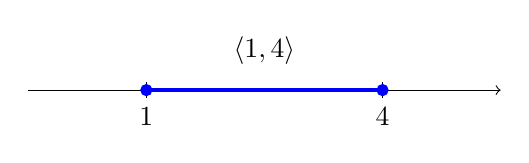
\begin{tikzpicture}[scale=1.0]
% Uzavřený interval [a,b]
\draw[->] (-0.5,0) -- (5.5,0);
\foreach \x in {1,4}
    \draw (\x,0.1) -- (\x,-0.1) node[below]{$\x$};
\draw[very thick,blue] (1,0) -- (4,0);
\filldraw[blue] (1,0) circle (2pt);
\filldraw[blue] (4,0) circle (2pt);
\node[above] at (2.5,0.2) {$\langle 1,4 \rangle$};
\end{tikzpicture}

\centering
{\small Interval obsahuje body $1$ i $4$.}
\end{minipage}\hfill
\begin{minipage}{0.45\textwidth}
\begin{tikzpicture}[scale=1.0]
% Otevřený interval (a,b)
\draw[->] (-0.5,0) -- (5.5,0);
\foreach \x in {1,4}
    \draw (\x,0.1) -- (\x,-0.1) node[below]{$\x$};
\draw[very thick,pastelorange!70!black] (1,0) -- (4,0);
\draw[pastelorange!70!black,very thick,fill=white] (1,0) circle (2pt);
\draw[pastelorange!70!black,very thick,fill=white] (4,0) circle (2pt);
\node[above] at (2.5,0.2) {$(1,4)$};
\end{tikzpicture}

\centering
{\small Interval neobsahuje body $1$ ani $4$.}
\end{minipage}

\vspace{1cm}

\begin{minipage}{0.45\textwidth}
\begin{tikzpicture}[scale=1.0]
% [a,b)
\draw[->] (-0.5,0) -- (5.5,0);
\foreach \x in {1,4}
    \draw (\x,0.1) -- (\x,-0.1) node[below]{$\x$};
\draw[very thick, pastelblue!70!black] (1,0) -- (4,0);
\filldraw[pastelblue!70!black] (1,0) circle (2pt);
\draw[pastelblue!70!black,very thick,fill=white] (4,0) circle (2pt);
\node[above] at (2.5,0.2) {$\langle 1,4)$};
\end{tikzpicture}

\centering
{\small Interval obsahuje bod $1$, ale neobsahuje bod $4$.}
\end{minipage}\hfill
\begin{minipage}{0.45\textwidth}
\begin{tikzpicture}[scale=1.0]
% (a,b]
\draw[->] (-0.5,0) -- (5.5,0);
\foreach \x in {1,4}
    \draw (\x,0.1) -- (\x,-0.1) node[below]{$\x$};
\draw[very thick,pastelgreen!70!black] (1,0) -- (4,0);
\draw[pastelgreen!70!black,very thick,fill=white] (1,0) circle (2pt);
\filldraw[pastelgreen!70!black] (4,0) circle (2pt);
\node[above] at (2.5,0.2) {$(1,4 \rangle$};
\end{tikzpicture}

\centering
{\small Interval neobsahuje bod $1$, ale obsahuje bod $4$.}
\end{minipage}
\end{center}


\newpage
\subsection*{Absolutní hodnota}

\begin{definitionbox}
\textbf{Absolutní hodnota} reálného čísla $a$ vyjadřuje \textbf{vzdálenost bodu $a$ od nuly na číselné ose}.  
Značí se svislými čarami $|a|$ a je vždy nezáporná. Formálně platí:
\[
|a| =
\begin{cases}
a, & \text{pokud } a \geq 0, \\
-a, & \text{pokud } a < 0.
\end{cases}
\]
\end{definitionbox}

\begin{notebox}
Například:  
\begin{itemize}
    \item Je-li $a=3$, pak $|a| = |3| = 3$, protože $a \geq 0$.  
    \item Je-li $a=-5$, pak $|a| = |-5| = -(-5) = 5$, protože $a < 0$.  
\end{itemize}
Absolutní hodnota tedy vždy vrací nezáporné číslo – představuje vzdálenost od nuly bez ohledu na směr.
\end{notebox}

Pro každá reálná čísla $a, b \in \mathbb{R}$ platí následující vlastnosti absolutní hodnoty:
\begin{center}
    $\left\lvert a \right\rvert = \sqrt{a^2}$ \\ 
    $\left\lvert a \right\rvert \geq 0$  \\
    $\left\lvert a \right\rvert = 0 \;\;\Leftrightarrow\;\; a = 0$  \\
    $\left\lvert -a \right\rvert = \left\lvert a \right\rvert$  \\
    $\left\lvert ab \right\rvert = \left\lvert a \right\rvert \cdot \left\lvert b \right\rvert$  \\
    $\left\lvert \tfrac{a}{b} \right\rvert = \tfrac{\left\lvert a \right\rvert}{\left\lvert b \right\rvert}, \;\; b \neq 0$  \\
    $\left\lvert a+b \right\rvert \leq \left\lvert a \right\rvert + \left\lvert b \right\rvert \quad$ (tzv. \textbf{trojúhelníková nerovnost})  \\
    $\left\lvert a-b \right\rvert = 0 \;\;\Leftrightarrow\;\; a = b$  \\

\end{center}


\exercisepart

\setcounter{section}{1}
\begin{exercise}[Rozdíl přirozených čísel]
Za jakých podmínek je rozdíl $a-b$ dvou přirozených čísel $a, b \in \mathbb{N}$ opět přirozené číslo?
\end{exercise}

\setcounter{section}{2}
\begin{exercise}[Úsporné počítání]
Za použití asociativity a komutativity sčítání nebo násobení vypočítejte co „nejúsporněji“:  
\begin{enumerate}[label=\alph*)]
    \item $28+33+7+22$  
    \item $31+16+49+64$  
    \item $5 \cdot 327 \cdot 2$  
    \item $4 \cdot 129 \cdot 25$  
    \item $125 \cdot 48 \cdot 2$  
    \item $50+37+63+150$  
\end{enumerate}
\end{exercise}

\begin{exercise}[Distributivita]
Využitím distributivity upravte a vypočítejte:  
\begin{enumerate}[label=\alph*)]
    \item $3 \cdot 658 + 7 \cdot 658$  
    \item $2 \cdot 10^3 + 3 \cdot 10^3$  
    \item $2 \cdot 10^3 + 3 \cdot 10^4$  
\end{enumerate}
\end{exercise}

\begin{exercise}[Opačná čísla]
Najděte čísla opačná k číslům:  
$7, \; -3, \; 0, \; a, \; -b, \; (x+5)$.
\end{exercise}

\begin{exercise}[Počítání zpaměti]
Vypočítejte zpaměti:  
\begin{tasks}(3) % číslo = počet sloupců
    \task $8 - (-7) - (7-3)$  
    \task $25 - (14 - 9)$  
    \task $-12 - (-8) + 5$  
    \task $(20-15) - (7-2)$  
    \task $50 - (20 - 17)$  
    \task $-5 - (3 - (-2))$  
    \task $(10-3) - (4-9)$  
    \task $100 - (75 - 20)$  
    \task $-\{-[-(-5)]\}+\{-[-(-5)]\}$
\end{tasks}
\end{exercise}

\newpage
\setcounter{section}{3}
\begin{exercise}[Základní tvar zlomku]
Zapište daná racionální čísla v \textbf{základním tvaru}:
\begin{tasks}(3)
    \task $\dfrac{180}{252}$
    \task $-\dfrac{108}{144}$
    \task $\dfrac{462}{1078}$
    \task $-\dfrac{840}{1980}$
    \task $\dfrac{918}{1530}$
    \task $-\dfrac{1287}{1716}$
\end{tasks}
\end{exercise}

\begin{exercise}[Převody zápisů racionálních čísel]
Převeďte čísla na zlomky, desetinné a složené čísla:
\begin{tasks}(3)
    \task $2\tfrac{3}{8}$
    \task $5\tfrac{7}{12}$
    \task $1.75$
    \task $0.04$
    \task $0.\overline{27}$
    \task $-1.2\overline{3}$
\end{tasks}
\end{exercise}

\begin{exercise}[Porovnávání zlomků]
Porovnejte dvojice zlomků ($<$, $>$, $=$):
\begin{tasks}(4)
    \task $\dfrac{1}{2}\ a \;\dfrac{3}{5}$
    \task $\dfrac{3}{7}\ a \;\dfrac{5}{7}$
    \task $\dfrac{2}{3}\ a \;\dfrac{4}{7}$
    \task $\dfrac{2}{3}\ a \;\dfrac{9}{11}$
    \task $\dfrac{10}{13}\ a \;\dfrac{18}{23}$
    \task $\dfrac{12}{18}\ a \;\dfrac{4}{6}$
    \task $\dfrac{11}{16}\ a \;\dfrac{32}{47}$
    \task $\dfrac{19}{45}\ a \;\dfrac{17}{40}$
    \task $\dfrac{23}{56}\ a \;\dfrac{11}{27}$
    \task $\dfrac{22}{7}\ a \;\dfrac{355}{113}$
    \task $\dfrac{333}{106}\ a \;\dfrac{355}{113}$
    \task $\dfrac{11}{32}\ a \;0,34$
\end{tasks}
\end{exercise}

\begin{exercise}[Počítání se zlomky]
Vypočítejte:
\begin{tasks}(2)
    \task $\dfrac{3}{4}+\dfrac{5}{8}$
    \task $\dfrac{7}{9}-\dfrac{2}{3}$
    \task $\dfrac{5}{12}+\dfrac{7}{18}$
    \task $\dfrac{11}{15}-\dfrac{4}{25}$
    \task $\dfrac{3}{10}\cdot\dfrac{5}{9}$
    \task $\dfrac{14}{27}\cdot\dfrac{9}{7}$
    \task $\left(\dfrac{2}{3}+\dfrac{1}{6}\right)-\dfrac{5}{12}$
    \task $\left[\dfrac{15}{4} \cdot \dfrac{2}{5} + \left(\dfrac{1}{2}-\dfrac{1}{3}\right)\cdot 2\right]:\dfrac{22}{3}$
\end{tasks}
\end{exercise}

\begin{exercise}[Težší počítání se zlomky]
    Vypočítejte:
    \begin{tasks}
        \task $\left[\dfrac{4}{12}\cdot\dfrac{6}{8}-2\left(\dfrac{2}{3}-\dfrac{1}{2}\right):\dfrac{4}{5}+\dfrac{2}{3} \right]\cdot\left[\dfrac{7}{6}\cdot\dfrac{15}{49}:\dfrac{10}{21}+\dfrac{5}{4}\right]$
    \end{tasks}
\end{exercise}

\setcounter{section}{4}

\begin{exercise}[Usmerňování zlomků]
    Usměrni zlomky:
    \begin{tasks}(4)
        \task $\dfrac{1}{\sqrt{3}}$
        \task $\dfrac{2}{\sqrt{2}}$
        \task $\dfrac{5}{\sqrt{5}}$
        \task $\dfrac{3}{2\sqrt{3}}$
        \task $\dfrac{9}{\sqrt{18}}$
        \task $\dfrac{1}{\sqrt[3]{2}}$
        \task $\dfrac{1}{\sqrt[3]{3}}$
        \task $\dfrac{1}{\sqrt[3]{18}}$
    \end{tasks}
\end{exercise}

\begin{exercise}[Usmerňování zlomků]
    Usměrni zlomky:
    \begin{tasks}(4)
        \task $\dfrac{1}{\sqrt{2}-1}$
        \task $\dfrac{1}{\sqrt{3}-1}$
        \task $\dfrac{2}{\sqrt{3}-1}$
        \task $\dfrac{1}{\sqrt{2}+1}$
        \task $\dfrac{\sqrt{3}}{1-\sqrt{5}}$
        \task $\dfrac{3}{\sqrt{5}+\sqrt{2}}$
        \task $\dfrac{\sqrt{2}}{\sqrt{2}+\sqrt{3}}$
        \task $\dfrac{1}{1+\sqrt{2}-1\sqrt{3}}$
    \end{tasks}
\end{exercise}

\begin{exercise}[Těžší porovnávání zlomků]
    Porovnejte:
    \begin{tasks}
        \task $\dfrac{\sqrt{3}}{\sqrt{2}} + \dfrac{\sqrt{5}}{\sqrt{3}} \;  a \; 1 + \dfrac{\sqrt{2}}{\sqrt{3}}$
    \end{tasks}
\end{exercise}
\setcounter{section}{5}

\begin{exercise}[Počítání s odmocninami]
    UVypočítejte:
    \begin{tasks}(3)
        \task $\left\lvert 3\right\rvert$
        \task $\left\lvert -1,5\right\rvert$
        \task $\left\lvert 9-2\right\rvert-\left\lvert -15-(-3)\right\rvert$
        \task $\left\lvert 7-\left\lvert 4-11\right\rvert\right\rvert$
        \task $\left\lvert 2-\sqrt{3}\right\rvert$
        \task $\left\lvert 1-\sqrt{2}\right\rvert$
    \end{tasks}
\end{exercise}

\begin{exercise}[Počítání s odmocninami]
    UVypočítejte:
    \begin{tasks}(2)
        \task $\left\lvert -2+\left\lvert -3\right\rvert\right\rvert$
        \task $\left\lvert -5+(-2)\left\lvert2 -3\right\rvert\right\rvert-8$
        \task $\left\lvert 2-\left\lvert3\right\rvert+4\cdot \left\lvert -2\right\rvert\right\rvert - \left\lvert3\cdot(-2) \right\rvert$
    \end{tasks}
\end{exercise}

\begin{exercise}[Absolutní hodnota na číselné ose]
    Na číselné ose vyznač pro jaké všechna reálný čísla platí:
    \begin{tasks}(2)
        \task $\left\lvert x-2\right\rvert = 3$
        \task $\left\lvert x-1\right\rvert > 1$
        \task $\left\lvert x+1\right\rvert \leq 2$
        \task $\left\lvert 1-x\right\rvert \leq 2$
        \task $\left\lvert x-\sqrt{2}\right\rvert < 2$
        \task $\left\lvert x-0,5\right\rvert \leq 1,5$
    \end{tasks}
\end{exercise}

\end{document}
